        \clearpage
        \begin{figure*}[ht]
            \pdfbookmark[2]{ID 01}{figure_id_01}
        	\centering
            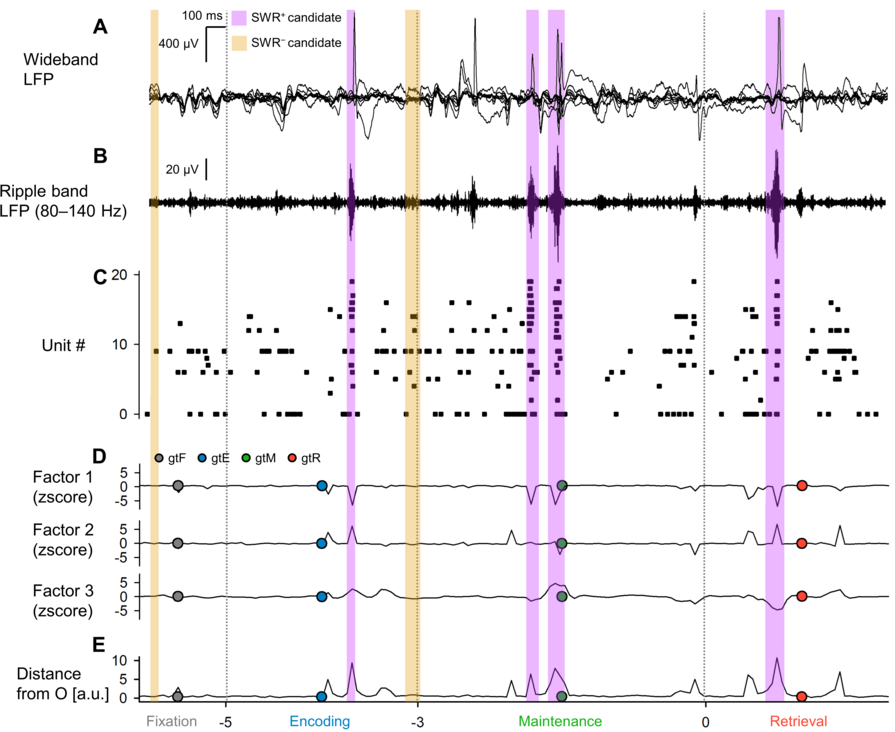
\includegraphics[width=1\textwidth]{./src/figures/.png/Figure_ID_01.png}
        	\caption{\textbf{
Local field potential (LFP), multiunit activity, and neural trajectory of the hippocampus during a modified Sternberg task
}
\smallskip
\\
\textbf{\textit{A.}} Wideband LFP Trace: Displaying the intracranial encephalogram (iEEG) data for subject \#6, session \#2, trial \#5, located in the left hippocampal head. This trace showcases the varying phases of the modified Sternberg working memory task, including fixation (\textit{gray}, 1 s), encoding (\textit{blue}, 2 s), maintenance (\textit{green}, 3 s), and retrieval (\textit{red}, 2 s). \textbf{\textit{B.}} Ripple Band LFP: This presents the LFP trace in the ripple frequency band from the same trial and session. \textbf{\textit{C.}} Multiunit Spike Raster: A plot illustrating multiunit spikes recorded during the mentioned trial. \textbf{\textit{D.}} Neural Trajectory Factors: Depicting the first three factors of the hippocampal trajectory for the trial, determined by Gaussian-process factor analysis on spike counts with 50-ms bins. The dot circles signify the geometric median coordinates for each of the four task phases. \textbf{\textit{E.}} Trajectory Distance Analysis: Shows the distance of the initial three trajectory factors from the origin ($O$). Note that highlighted rectangles overlaying the figure indicate the timings for SWR$^+$ candidates (in \textit{purple}) and SWR$^-$ candidates (in \textit{yellow}).
}
% width=1\textwidth
        	\label{fig:01}
        \end{figure*}
